% Options for packages loaded elsewhere
\PassOptionsToPackage{unicode}{hyperref}
\PassOptionsToPackage{hyphens}{url}
\PassOptionsToPackage{dvipsnames,svgnames,x11names}{xcolor}
%
\documentclass[
  letterpaper,
  DIV=11,
  numbers=noendperiod]{scrartcl}

\usepackage{amsmath,amssymb}
\usepackage{lmodern}
\usepackage{iftex}
\ifPDFTeX
  \usepackage[T1]{fontenc}
  \usepackage[utf8]{inputenc}
  \usepackage{textcomp} % provide euro and other symbols
\else % if luatex or xetex
  \usepackage{unicode-math}
  \defaultfontfeatures{Scale=MatchLowercase}
  \defaultfontfeatures[\rmfamily]{Ligatures=TeX,Scale=1}
\fi
% Use upquote if available, for straight quotes in verbatim environments
\IfFileExists{upquote.sty}{\usepackage{upquote}}{}
\IfFileExists{microtype.sty}{% use microtype if available
  \usepackage[]{microtype}
  \UseMicrotypeSet[protrusion]{basicmath} % disable protrusion for tt fonts
}{}
\makeatletter
\@ifundefined{KOMAClassName}{% if non-KOMA class
  \IfFileExists{parskip.sty}{%
    \usepackage{parskip}
  }{% else
    \setlength{\parindent}{0pt}
    \setlength{\parskip}{6pt plus 2pt minus 1pt}}
}{% if KOMA class
  \KOMAoptions{parskip=half}}
\makeatother
\usepackage{xcolor}
\setlength{\emergencystretch}{3em} % prevent overfull lines
\setcounter{secnumdepth}{-\maxdimen} % remove section numbering
% Make \paragraph and \subparagraph free-standing
\ifx\paragraph\undefined\else
  \let\oldparagraph\paragraph
  \renewcommand{\paragraph}[1]{\oldparagraph{#1}\mbox{}}
\fi
\ifx\subparagraph\undefined\else
  \let\oldsubparagraph\subparagraph
  \renewcommand{\subparagraph}[1]{\oldsubparagraph{#1}\mbox{}}
\fi

\usepackage{color}
\usepackage{fancyvrb}
\newcommand{\VerbBar}{|}
\newcommand{\VERB}{\Verb[commandchars=\\\{\}]}
\DefineVerbatimEnvironment{Highlighting}{Verbatim}{commandchars=\\\{\}}
% Add ',fontsize=\small' for more characters per line
\usepackage{framed}
\definecolor{shadecolor}{RGB}{241,243,245}
\newenvironment{Shaded}{\begin{snugshade}}{\end{snugshade}}
\newcommand{\AlertTok}[1]{\textcolor[rgb]{0.68,0.00,0.00}{#1}}
\newcommand{\AnnotationTok}[1]{\textcolor[rgb]{0.37,0.37,0.37}{#1}}
\newcommand{\AttributeTok}[1]{\textcolor[rgb]{0.40,0.45,0.13}{#1}}
\newcommand{\BaseNTok}[1]{\textcolor[rgb]{0.68,0.00,0.00}{#1}}
\newcommand{\BuiltInTok}[1]{\textcolor[rgb]{0.00,0.23,0.31}{#1}}
\newcommand{\CharTok}[1]{\textcolor[rgb]{0.13,0.47,0.30}{#1}}
\newcommand{\CommentTok}[1]{\textcolor[rgb]{0.37,0.37,0.37}{#1}}
\newcommand{\CommentVarTok}[1]{\textcolor[rgb]{0.37,0.37,0.37}{\textit{#1}}}
\newcommand{\ConstantTok}[1]{\textcolor[rgb]{0.56,0.35,0.01}{#1}}
\newcommand{\ControlFlowTok}[1]{\textcolor[rgb]{0.00,0.23,0.31}{#1}}
\newcommand{\DataTypeTok}[1]{\textcolor[rgb]{0.68,0.00,0.00}{#1}}
\newcommand{\DecValTok}[1]{\textcolor[rgb]{0.68,0.00,0.00}{#1}}
\newcommand{\DocumentationTok}[1]{\textcolor[rgb]{0.37,0.37,0.37}{\textit{#1}}}
\newcommand{\ErrorTok}[1]{\textcolor[rgb]{0.68,0.00,0.00}{#1}}
\newcommand{\ExtensionTok}[1]{\textcolor[rgb]{0.00,0.23,0.31}{#1}}
\newcommand{\FloatTok}[1]{\textcolor[rgb]{0.68,0.00,0.00}{#1}}
\newcommand{\FunctionTok}[1]{\textcolor[rgb]{0.28,0.35,0.67}{#1}}
\newcommand{\ImportTok}[1]{\textcolor[rgb]{0.00,0.46,0.62}{#1}}
\newcommand{\InformationTok}[1]{\textcolor[rgb]{0.37,0.37,0.37}{#1}}
\newcommand{\KeywordTok}[1]{\textcolor[rgb]{0.00,0.23,0.31}{#1}}
\newcommand{\NormalTok}[1]{\textcolor[rgb]{0.00,0.23,0.31}{#1}}
\newcommand{\OperatorTok}[1]{\textcolor[rgb]{0.37,0.37,0.37}{#1}}
\newcommand{\OtherTok}[1]{\textcolor[rgb]{0.00,0.23,0.31}{#1}}
\newcommand{\PreprocessorTok}[1]{\textcolor[rgb]{0.68,0.00,0.00}{#1}}
\newcommand{\RegionMarkerTok}[1]{\textcolor[rgb]{0.00,0.23,0.31}{#1}}
\newcommand{\SpecialCharTok}[1]{\textcolor[rgb]{0.37,0.37,0.37}{#1}}
\newcommand{\SpecialStringTok}[1]{\textcolor[rgb]{0.13,0.47,0.30}{#1}}
\newcommand{\StringTok}[1]{\textcolor[rgb]{0.13,0.47,0.30}{#1}}
\newcommand{\VariableTok}[1]{\textcolor[rgb]{0.07,0.07,0.07}{#1}}
\newcommand{\VerbatimStringTok}[1]{\textcolor[rgb]{0.13,0.47,0.30}{#1}}
\newcommand{\WarningTok}[1]{\textcolor[rgb]{0.37,0.37,0.37}{\textit{#1}}}

\providecommand{\tightlist}{%
  \setlength{\itemsep}{0pt}\setlength{\parskip}{0pt}}\usepackage{longtable,booktabs,array}
\usepackage{calc} % for calculating minipage widths
% Correct order of tables after \paragraph or \subparagraph
\usepackage{etoolbox}
\makeatletter
\patchcmd\longtable{\par}{\if@noskipsec\mbox{}\fi\par}{}{}
\makeatother
% Allow footnotes in longtable head/foot
\IfFileExists{footnotehyper.sty}{\usepackage{footnotehyper}}{\usepackage{footnote}}
\makesavenoteenv{longtable}
\usepackage{graphicx}
\makeatletter
\def\maxwidth{\ifdim\Gin@nat@width>\linewidth\linewidth\else\Gin@nat@width\fi}
\def\maxheight{\ifdim\Gin@nat@height>\textheight\textheight\else\Gin@nat@height\fi}
\makeatother
% Scale images if necessary, so that they will not overflow the page
% margins by default, and it is still possible to overwrite the defaults
% using explicit options in \includegraphics[width, height, ...]{}
\setkeys{Gin}{width=\maxwidth,height=\maxheight,keepaspectratio}
% Set default figure placement to htbp
\makeatletter
\def\fps@figure{htbp}
\makeatother

\KOMAoption{captions}{tableheading}
\makeatletter
\makeatother
\makeatletter
\makeatother
\makeatletter
\@ifpackageloaded{caption}{}{\usepackage{caption}}
\AtBeginDocument{%
\ifdefined\contentsname
  \renewcommand*\contentsname{Table of contents}
\else
  \newcommand\contentsname{Table of contents}
\fi
\ifdefined\listfigurename
  \renewcommand*\listfigurename{List of Figures}
\else
  \newcommand\listfigurename{List of Figures}
\fi
\ifdefined\listtablename
  \renewcommand*\listtablename{List of Tables}
\else
  \newcommand\listtablename{List of Tables}
\fi
\ifdefined\figurename
  \renewcommand*\figurename{Figure}
\else
  \newcommand\figurename{Figure}
\fi
\ifdefined\tablename
  \renewcommand*\tablename{Table}
\else
  \newcommand\tablename{Table}
\fi
}
\@ifpackageloaded{float}{}{\usepackage{float}}
\floatstyle{ruled}
\@ifundefined{c@chapter}{\newfloat{codelisting}{h}{lop}}{\newfloat{codelisting}{h}{lop}[chapter]}
\floatname{codelisting}{Listing}
\newcommand*\listoflistings{\listof{codelisting}{List of Listings}}
\makeatother
\makeatletter
\@ifpackageloaded{caption}{}{\usepackage{caption}}
\@ifpackageloaded{subcaption}{}{\usepackage{subcaption}}
\makeatother
\makeatletter
\@ifpackageloaded{tcolorbox}{}{\usepackage[many]{tcolorbox}}
\makeatother
\makeatletter
\@ifundefined{shadecolor}{\definecolor{shadecolor}{rgb}{.97, .97, .97}}
\makeatother
\makeatletter
\makeatother
\ifLuaTeX
  \usepackage{selnolig}  % disable illegal ligatures
\fi
\IfFileExists{bookmark.sty}{\usepackage{bookmark}}{\usepackage{hyperref}}
\IfFileExists{xurl.sty}{\usepackage{xurl}}{} % add URL line breaks if available
\urlstyle{same} % disable monospaced font for URLs
\hypersetup{
  pdftitle={Class 6 R Functions},
  colorlinks=true,
  linkcolor={blue},
  filecolor={Maroon},
  citecolor={Blue},
  urlcolor={Blue},
  pdfcreator={LaTeX via pandoc}}

\title{Class 6 R Functions}
\author{}
\date{}

\begin{document}
\maketitle
\ifdefined\Shaded\renewenvironment{Shaded}{\begin{tcolorbox}[breakable, frame hidden, boxrule=0pt, enhanced, borderline west={3pt}{0pt}{shadecolor}, interior hidden, sharp corners]}{\end{tcolorbox}}\fi

We are looking at \emph{R Functions} and how to write them.

\begin{quote}
Q1. Write a function grade() to determine an overall grade from a vector
of student homework assignment scores dropping the lowest single score.
If a student misses a homework (i.e.~has an NA value) this can be used
as a score to be potentially dropped. Your final function should be
adquately explained with code comments and be able to work on an example
class gradebook such as this one in CSV format:
``https://tinyurl.com/gradeinput''
\end{quote}

\begin{Shaded}
\begin{Highlighting}[]
\CommentTok{\# Example input vectors to start with}
\NormalTok{student1 }\OtherTok{\textless{}{-}} \FunctionTok{c}\NormalTok{(}\DecValTok{100}\NormalTok{, }\DecValTok{100}\NormalTok{, }\DecValTok{100}\NormalTok{, }\DecValTok{100}\NormalTok{, }\DecValTok{100}\NormalTok{, }\DecValTok{100}\NormalTok{, }\DecValTok{100}\NormalTok{, }\DecValTok{90}\NormalTok{)}
\NormalTok{student2 }\OtherTok{\textless{}{-}} \FunctionTok{c}\NormalTok{(}\DecValTok{100}\NormalTok{, }\ConstantTok{NA}\NormalTok{, }\DecValTok{90}\NormalTok{, }\DecValTok{90}\NormalTok{, }\DecValTok{90}\NormalTok{, }\DecValTok{90}\NormalTok{, }\DecValTok{97}\NormalTok{, }\DecValTok{80}\NormalTok{)}
\NormalTok{student3 }\OtherTok{\textless{}{-}} \FunctionTok{c}\NormalTok{(}\DecValTok{90}\NormalTok{, }\ConstantTok{NA}\NormalTok{, }\ConstantTok{NA}\NormalTok{, }\ConstantTok{NA}\NormalTok{, }\ConstantTok{NA}\NormalTok{, }\ConstantTok{NA}\NormalTok{, }\ConstantTok{NA}\NormalTok{, }\ConstantTok{NA}\NormalTok{)}
\end{Highlighting}
\end{Shaded}

Follow the guidelines from class - Write a working snippet of code that
solves simple version of problem

\begin{Shaded}
\begin{Highlighting}[]
\CommentTok{\# mean()}
\NormalTok{student1 }\OtherTok{\textless{}{-}} \FunctionTok{c}\NormalTok{(}\DecValTok{100}\NormalTok{, }\DecValTok{100}\NormalTok{, }\DecValTok{100}\NormalTok{, }\DecValTok{100}\NormalTok{, }\DecValTok{100}\NormalTok{, }\DecValTok{100}\NormalTok{, }\DecValTok{100}\NormalTok{, }\DecValTok{90}\NormalTok{)}


\FunctionTok{mean}\NormalTok{(student1)}
\end{Highlighting}
\end{Shaded}

\begin{verbatim}
[1] 98.75
\end{verbatim}

Must drop lowest score. Must identify lowest score in vector.

\begin{Shaded}
\begin{Highlighting}[]
\CommentTok{\# Which element of vector is the lowest?}
\FunctionTok{which.min}\NormalTok{(student1)}
\end{Highlighting}
\end{Shaded}

\begin{verbatim}
[1] 8
\end{verbatim}

Time to drop lowest score from grade calculation

\begin{Shaded}
\begin{Highlighting}[]
\CommentTok{\# return everything but the }
\CommentTok{\# eighth element in the vector}
\NormalTok{student1[}\SpecialCharTok{{-}}\DecValTok{8}\NormalTok{]}
\end{Highlighting}
\end{Shaded}

\begin{verbatim}
[1] 100 100 100 100 100 100 100
\end{verbatim}

Now we use which.min() to return all other elements of vector minus the
smallest one

\begin{Shaded}
\begin{Highlighting}[]
\NormalTok{student1[}\SpecialCharTok{{-}}\FunctionTok{which.min}\NormalTok{(student1)]}
\end{Highlighting}
\end{Shaded}

\begin{verbatim}
[1] 100 100 100 100 100 100 100
\end{verbatim}

\begin{Shaded}
\begin{Highlighting}[]
\CommentTok{\# average of student 1 with lowest score dropped }
\CommentTok{\# first working snippet of code}
\FunctionTok{mean}\NormalTok{( student1[}\SpecialCharTok{{-}}\FunctionTok{which.min}\NormalTok{(student1)] )}
\end{Highlighting}
\end{Shaded}

\begin{verbatim}
[1] 100
\end{verbatim}

Now other students??

using na.rm=TRUE only would be an unfair grading approach

\begin{Shaded}
\begin{Highlighting}[]
\NormalTok{student2 }\OtherTok{\textless{}{-}} \FunctionTok{c}\NormalTok{(}\DecValTok{100}\NormalTok{, }\ConstantTok{NA}\NormalTok{, }\DecValTok{90}\NormalTok{, }\DecValTok{90}\NormalTok{, }\DecValTok{90}\NormalTok{, }\DecValTok{90}\NormalTok{, }\DecValTok{97}\NormalTok{, }\DecValTok{80}\NormalTok{)}
\FunctionTok{mean}\NormalTok{(student2, }\AttributeTok{na.rm=}\ConstantTok{TRUE}\NormalTok{)}
\end{Highlighting}
\end{Shaded}

\begin{verbatim}
[1] 91
\end{verbatim}

\begin{Shaded}
\begin{Highlighting}[]
\NormalTok{student3 }\OtherTok{\textless{}{-}} \FunctionTok{c}\NormalTok{(}\DecValTok{90}\NormalTok{, }\ConstantTok{NA}\NormalTok{, }\ConstantTok{NA}\NormalTok{, }\ConstantTok{NA}\NormalTok{, }\ConstantTok{NA}\NormalTok{, }\ConstantTok{NA}\NormalTok{, }\ConstantTok{NA}\NormalTok{, }\ConstantTok{NA}\NormalTok{)}
\FunctionTok{mean}\NormalTok{(student3, }\AttributeTok{na.rm=}\ConstantTok{TRUE}\NormalTok{)}
\end{Highlighting}
\end{Shaded}

\begin{verbatim}
[1] 90
\end{verbatim}

One approach cold be to replace all NA values with zero

First, need to be able to find NA values of vector.

\begin{Shaded}
\begin{Highlighting}[]
\NormalTok{student2 }\OtherTok{\textless{}{-}} \FunctionTok{c}\NormalTok{(}\DecValTok{100}\NormalTok{, }\ConstantTok{NA}\NormalTok{, }\DecValTok{90}\NormalTok{, }\DecValTok{90}\NormalTok{, }\DecValTok{90}\NormalTok{, }\DecValTok{90}\NormalTok{, }\DecValTok{97}\NormalTok{, }\DecValTok{80}\NormalTok{)}
\NormalTok{x }\OtherTok{\textless{}{-}}\NormalTok{ student2}

\CommentTok{\#tells us if any values in vector is NA}
\FunctionTok{is.na}\NormalTok{(x)}
\end{Highlighting}
\end{Shaded}

\begin{verbatim}
[1] FALSE  TRUE FALSE FALSE FALSE FALSE FALSE FALSE
\end{verbatim}

\begin{Shaded}
\begin{Highlighting}[]
\CommentTok{\#tells us location of NA values in vector}
\FunctionTok{which}\NormalTok{(}\FunctionTok{is.na}\NormalTok{(x))}
\end{Highlighting}
\end{Shaded}

\begin{verbatim}
[1] 2
\end{verbatim}

NA elements identified. Time to ``mask'' them with value of 0 for
calculations.

\begin{Shaded}
\begin{Highlighting}[]
\CommentTok{\# Changing all NA elements in vector "x" to 0}
\NormalTok{x[}\FunctionTok{is.na}\NormalTok{(x)] }\OtherTok{\textless{}{-}} \DecValTok{0}
\NormalTok{x}
\end{Highlighting}
\end{Shaded}

\begin{verbatim}
[1] 100   0  90  90  90  90  97  80
\end{verbatim}

\begin{Shaded}
\begin{Highlighting}[]
\FunctionTok{mean}\NormalTok{(x)}
\end{Highlighting}
\end{Shaded}

\begin{verbatim}
[1] 79.625
\end{verbatim}

Now need to be able to drop lowest score before calculating mean

\begin{Shaded}
\begin{Highlighting}[]
\NormalTok{x[}\FunctionTok{is.na}\NormalTok{(x)] }\OtherTok{\textless{}{-}} \DecValTok{0}
\FunctionTok{mean}\NormalTok{( x[}\SpecialCharTok{{-}}\FunctionTok{which.min}\NormalTok{(x)] )}
\end{Highlighting}
\end{Shaded}

\begin{verbatim}
[1] 91
\end{verbatim}

Our working snippet code

\begin{Shaded}
\begin{Highlighting}[]
\NormalTok{student3 }\OtherTok{\textless{}{-}} \FunctionTok{c}\NormalTok{(}\DecValTok{90}\NormalTok{, }\ConstantTok{NA}\NormalTok{, }\ConstantTok{NA}\NormalTok{, }\ConstantTok{NA}\NormalTok{, }\ConstantTok{NA}\NormalTok{, }\ConstantTok{NA}\NormalTok{, }\ConstantTok{NA}\NormalTok{, }\ConstantTok{NA}\NormalTok{)}
\NormalTok{x }\OtherTok{\textless{}{-}}\NormalTok{ student3}
\NormalTok{x[}\FunctionTok{is.na}\NormalTok{(x)] }\OtherTok{\textless{}{-}} \DecValTok{0}
\FunctionTok{mean}\NormalTok{( x[}\SpecialCharTok{{-}}\FunctionTok{which.min}\NormalTok{(x)] )}
\end{Highlighting}
\end{Shaded}

\begin{verbatim}
[1] 12.85714
\end{verbatim}

\hypertarget{function}{%
\subsection{Function}\label{function}}

Take the snippet and turn into function Every function has 3 parts

\begin{itemize}
\tightlist
\item
  A name, in this case `grade()'
\item
  Input arguments, in this case a vector of student numeric scores
\item
  The body, aka the working snippet
\end{itemize}

Using RStudio, will select `Code' \textgreater{} `Extract Function'

\begin{Shaded}
\begin{Highlighting}[]
\CommentTok{\#\textquotesingle{} Calculate average score from a vector of}
\CommentTok{\#\textquotesingle{} student scores while dropping the lowest score.}
\CommentTok{\#\textquotesingle{} Missing values are assigned value of 0.}
\CommentTok{\#\textquotesingle{}}
\CommentTok{\#\textquotesingle{} @param x A numeric vector of homework scores of a student}
\CommentTok{\#\textquotesingle{}}
\CommentTok{\#\textquotesingle{} @return Average score}
\CommentTok{\#\textquotesingle{} @examples}
\CommentTok{\#\textquotesingle{}  student \textless{}{-} c(100, NA, 90, 97}
\CommentTok{\#\textquotesingle{}  grade(student))}

\NormalTok{grade }\OtherTok{\textless{}{-}} \ControlFlowTok{function}\NormalTok{(x) \{}
  \CommentTok{\# mask NA with zero}
  \CommentTok{\# Treat NA as zero in calculation}
\NormalTok{  x[}\FunctionTok{is.na}\NormalTok{(x)] }\OtherTok{\textless{}{-}} \DecValTok{0}
  \CommentTok{\# Exclude lowest score from calculation}
  \FunctionTok{mean}\NormalTok{( x[}\SpecialCharTok{{-}}\FunctionTok{which.min}\NormalTok{(x)] )}
\NormalTok{\}}
\end{Highlighting}
\end{Shaded}

\begin{Shaded}
\begin{Highlighting}[]
\FunctionTok{grade}\NormalTok{(student1)}
\end{Highlighting}
\end{Shaded}

\begin{verbatim}
[1] 100
\end{verbatim}

\begin{Shaded}
\begin{Highlighting}[]
\FunctionTok{grade}\NormalTok{(student2)}
\end{Highlighting}
\end{Shaded}

\begin{verbatim}
[1] 91
\end{verbatim}

\begin{Shaded}
\begin{Highlighting}[]
\FunctionTok{grade}\NormalTok{(student3)}
\end{Highlighting}
\end{Shaded}

\begin{verbatim}
[1] 12.85714
\end{verbatim}

It works!

Now we can use our function on class data in the CSV file:
``https://tinyurl.com/gradeinput''

\begin{Shaded}
\begin{Highlighting}[]
\NormalTok{url }\OtherTok{\textless{}{-}} \StringTok{"https://tinyurl.com/gradeinput"}
\NormalTok{gradebook }\OtherTok{\textless{}{-}} \FunctionTok{read.csv}\NormalTok{(url, }\AttributeTok{row.names =} \DecValTok{1}\NormalTok{)}
\end{Highlighting}
\end{Shaded}

\begin{Shaded}
\begin{Highlighting}[]
\FunctionTok{apply}\NormalTok{(gradebook, }\DecValTok{1}\NormalTok{, grade)}
\end{Highlighting}
\end{Shaded}

\begin{verbatim}
 student-1  student-2  student-3  student-4  student-5  student-6  student-7 
     91.75      82.50      84.25      84.25      88.25      89.00      94.00 
 student-8  student-9 student-10 student-11 student-12 student-13 student-14 
     93.75      87.75      79.00      86.00      91.75      92.25      87.75 
student-15 student-16 student-17 student-18 student-19 student-20 
     78.75      89.50      88.00      94.50      82.75      82.75 
\end{verbatim}

\begin{quote}
Q2. Who is the top scoring student overall in the gradebook?
\end{quote}

\begin{Shaded}
\begin{Highlighting}[]
\CommentTok{\# Apply calculations to value \textquotesingle{}results\textquotesingle{}}
\NormalTok{results }\OtherTok{\textless{}{-}} \FunctionTok{apply}\NormalTok{(gradebook, }\DecValTok{1}\NormalTok{, grade)}
\CommentTok{\# Sort the values by decreasing order}
\FunctionTok{sort}\NormalTok{(results, }\AttributeTok{decreasing =} \ConstantTok{TRUE}\NormalTok{)}
\end{Highlighting}
\end{Shaded}

\begin{verbatim}
student-18  student-7  student-8 student-13  student-1 student-12 student-16 
     94.50      94.00      93.75      92.25      91.75      91.75      89.50 
 student-6  student-5 student-17  student-9 student-14 student-11  student-3 
     89.00      88.25      88.00      87.75      87.75      86.00      84.25 
 student-4 student-19 student-20  student-2 student-10 student-15 
     84.25      82.75      82.75      82.50      79.00      78.75 
\end{verbatim}

\begin{Shaded}
\begin{Highlighting}[]
\FunctionTok{which.max}\NormalTok{(results)}
\end{Highlighting}
\end{Shaded}

\begin{verbatim}
student-18 
        18 
\end{verbatim}

\begin{quote}
Q3. Which homework was the toughest on the students?
\end{quote}

\begin{Shaded}
\begin{Highlighting}[]
\NormalTok{gradebook}
\end{Highlighting}
\end{Shaded}

\begin{verbatim}
           hw1 hw2 hw3 hw4 hw5
student-1  100  73 100  88  79
student-2   85  64  78  89  78
student-3   83  69  77 100  77
student-4   88  NA  73 100  76
student-5   88 100  75  86  79
student-6   89  78 100  89  77
student-7   89 100  74  87 100
student-8   89 100  76  86 100
student-9   86 100  77  88  77
student-10  89  72  79  NA  76
student-11  82  66  78  84 100
student-12 100  70  75  92 100
student-13  89 100  76 100  80
student-14  85 100  77  89  76
student-15  85  65  76  89  NA
student-16  92 100  74  89  77
student-17  88  63 100  86  78
student-18  91  NA 100  87 100
student-19  91  68  75  86  79
student-20  91  68  76  88  76
\end{verbatim}

\begin{Shaded}
\begin{Highlighting}[]
\NormalTok{avg.scores }\OtherTok{\textless{}{-}} \FunctionTok{apply}\NormalTok{(gradebook, }\DecValTok{2}\NormalTok{, mean, }\AttributeTok{na.rm =} \ConstantTok{TRUE}\NormalTok{)}
\NormalTok{avg.scores}
\end{Highlighting}
\end{Shaded}

\begin{verbatim}
     hw1      hw2      hw3      hw4      hw5 
89.00000 80.88889 80.80000 89.63158 83.42105 
\end{verbatim}

\begin{Shaded}
\begin{Highlighting}[]
\FunctionTok{which.min}\NormalTok{(avg.scores)}
\end{Highlighting}
\end{Shaded}

\begin{verbatim}
hw3 
  3 
\end{verbatim}

\begin{Shaded}
\begin{Highlighting}[]
\NormalTok{med.scores }\OtherTok{\textless{}{-}} \FunctionTok{apply}\NormalTok{(gradebook, }\DecValTok{2}\NormalTok{, median, }\AttributeTok{na.rm =} \ConstantTok{TRUE}\NormalTok{)}
\NormalTok{med.scores}
\end{Highlighting}
\end{Shaded}

\begin{verbatim}
 hw1  hw2  hw3  hw4  hw5 
89.0 72.5 76.5 88.0 78.0 
\end{verbatim}

\begin{Shaded}
\begin{Highlighting}[]
\FunctionTok{which.min}\NormalTok{(med.scores)}
\end{Highlighting}
\end{Shaded}

\begin{verbatim}
hw2 
  2 
\end{verbatim}

\begin{Shaded}
\begin{Highlighting}[]
\FunctionTok{boxplot}\NormalTok{(gradebook)}
\end{Highlighting}
\end{Shaded}

\begin{figure}[H]

{\centering 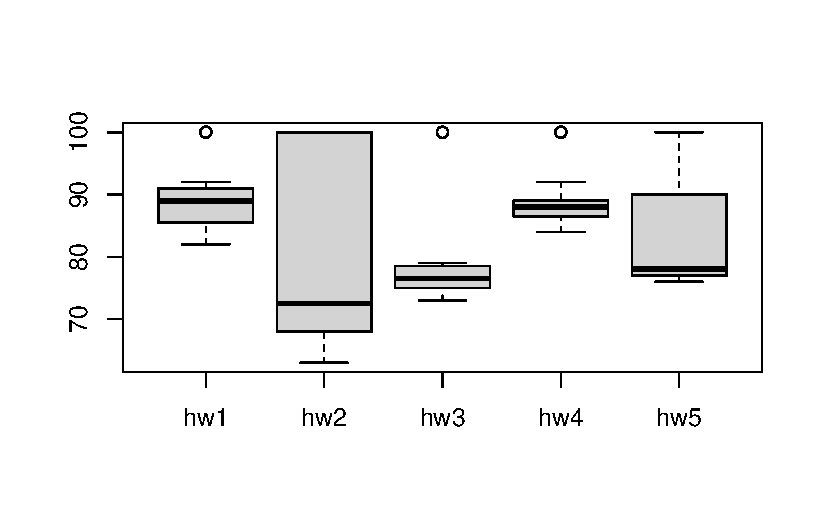
\includegraphics{class6wksheetstuff!!!_files/figure-pdf/unnamed-chunk-21-1.pdf}

}

\end{figure}



\end{document}
